\documentclass[convert]{standalone}

\usepackage{tikz}
\usetikzlibrary{backgrounds}
\usepgflibrary{shadings} 


\begin{document}


\begin{tabular}{cc}
  Vernal Equinox & Summer Solstice $(\alpha=-23.5\deg)$ \\
  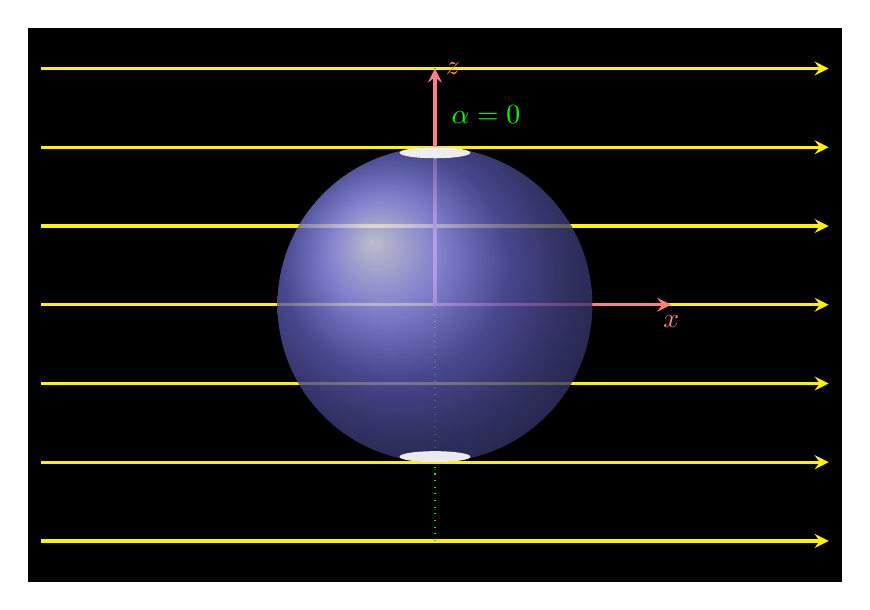
\begin{tikzpicture}[background rectangle/.style={fill=black}, show background
    rectangle,>=stealth]
    \node at (0,3.25) {};
    \node at (0,-3.25) {};
    \foreach \i in {-3,-2,...,3}{
      \draw[yellow,very thick,->] (-5,\i) -- (5,\i);
    }
    \draw[green, dotted] (0,-3) -- (0,3);
    \begin{scope}[red!50!white, very thick,rotate=0]
      \draw[->] (0,0) -- +(3,0) node[below]{$x$};
      \draw[->] (0,0) -- +(0,3) node[right]{$z$};
      \shade[ball color=blue!50!white,opacity=0.8] (0,0) circle (2);
      \fill[white,opacity=0.9] (0,1.93) ellipse (0.45 and 0.07);
      \fill[white,opacity=0.9] (0,-1.93) ellipse (0.45 and 0.07);
    \end{scope}
    \node at (75:2.5) [green]{$\alpha=0$};
  \end{tikzpicture}
                 &
                   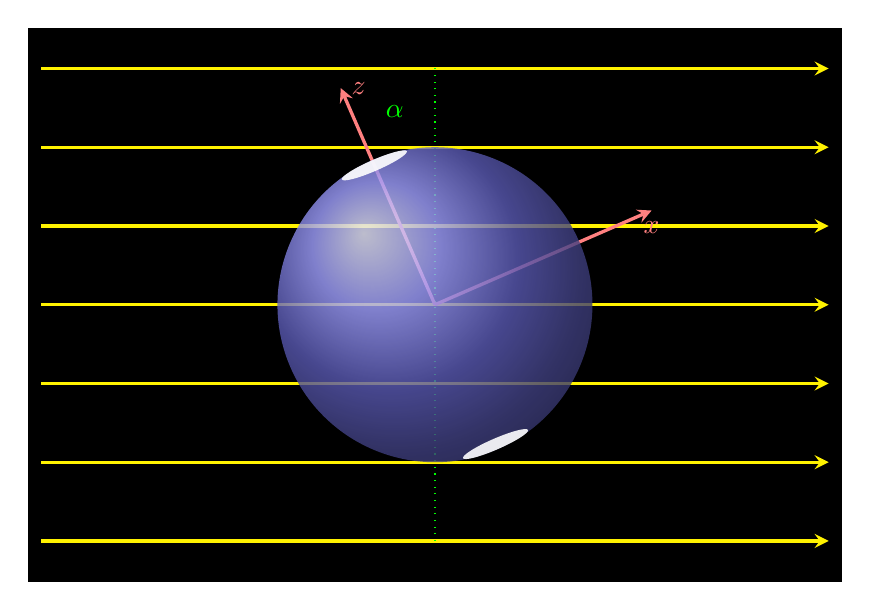
\begin{tikzpicture}[background rectangle/.style={fill=black},
                     show background rectangle,>=stealth]
                     \node at (0,3.25) {};
                     \node at (0,-3.25) {};
                     \foreach \i in {-3,-2,...,3}{
                       \draw[yellow,very thick,->] (-5,\i) -- (5,\i);
                     }
                     \draw[green, dotted] (0,-3) -- (0,3);
                     \begin{scope}[red!50!white, very thick,rotate=23.5]
                       \draw[->] (0,0) -- +(3,0) node[below]{$x$};
                       \draw[->] (0,0) -- +(0,3) node[right]{$z$};
                       \shade[ball color=blue!50!white,opacity=0.8] (0,0) circle (2);
                       \fill[white,opacity=0.9] (0,1.93) ellipse (0.45 and 0.07);
                       \fill[white,opacity=0.9] (0,-1.93) ellipse (0.45 and 0.07);
                     \end{scope}
                     \node at (101.75:2.5) [green]{$\alpha$};
                   \end{tikzpicture}
\\  
  Autumnal Equinox & Winter Solstice $(\alpha=+23.5\deg)$ \\
  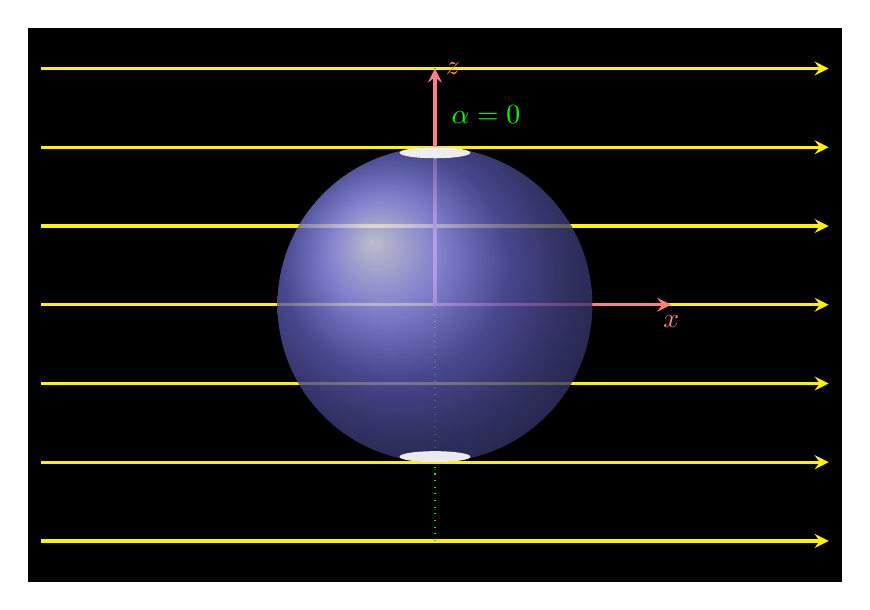
\begin{tikzpicture}[background rectangle/.style={fill=black}, show background rectangle,>=stealth]
    \node at (0,3.25) {};
    \node at (0,-3.25) {};
    \foreach \i in {-3,-2,...,3}{
      \draw[yellow,very thick,->] (-5,\i) -- (5,\i);
    }
    \draw[green, dotted] (0,-3) -- (0,3);
    \begin{scope}[red!50!white, very thick,rotate=0]
      \draw[->] (0,0) -- +(3,0) node[below]{$x$};
      \draw[->] (0,0) -- +(0,3) node[right]{$z$};
      \shade[ball color=blue!50!white,opacity=0.8] (0,0) circle (2);
      \fill[white,opacity=0.9] (0,1.93) ellipse (0.45 and 0.07);
      \fill[white,opacity=0.9] (0,-1.93) ellipse (0.45 and 0.07);
    \end{scope}
    \node at (75:2.5) [green]{$\alpha=0$};
  \end{tikzpicture}
                 &
                   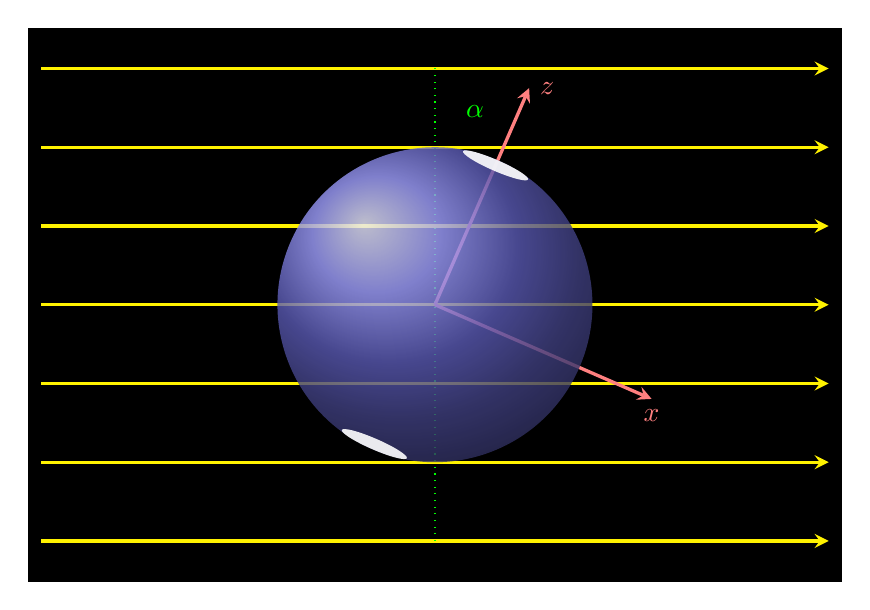
\begin{tikzpicture}[background rectangle/.style={fill=black},
                     show background rectangle,>=stealth]
                     \node at (0,3.25) {};
                     \node at (0,-3.25) {};
                     \foreach \i in {-3,-2,...,3}{
                       \draw[yellow,->,very thick] (-5,\i) -- (5,\i);
                     }
                     \draw[green, dotted] (0,-3) -- (0,3);
                     \begin{scope}[red!50!white, very thick,rotate=-23.5]
                       \draw[->] (0,0) -- +(3,0) node[below]{$x$};
                       \draw[->] (0,0) -- +(0,3) node[right]{$z$};
                       \shade[ball color=blue!50!white,opacity=0.8] (0,0) circle (2);
                       \fill[white,opacity=0.9] (0,1.93) ellipse (0.45 and 0.07);
                       \fill[white,opacity=0.9] (0,-1.93) ellipse (0.45 and 0.07);
                     \end{scope}
                     \node at (78.25:2.5) [green]{$\alpha$};
                   \end{tikzpicture}
\\
  
\end{tabular}

\end{document}